\chapter{Simple Models of the Cardiovascular System for Educational and Research Purposes}\label{app:simplemodelsd}
The paper \cite{Kulhanek2014mefanet} published as
 
\bibentry{Kulhanek2014mefanet}

Available online at \url{http://mj.mefanet.cz/mj-04140914}

Author of this thesis proposed and implemented several models related to cardiovascular system in Modelica language. Other co-authors updated general library for modeling physiology and proposed utilization of the models in educational simulators.

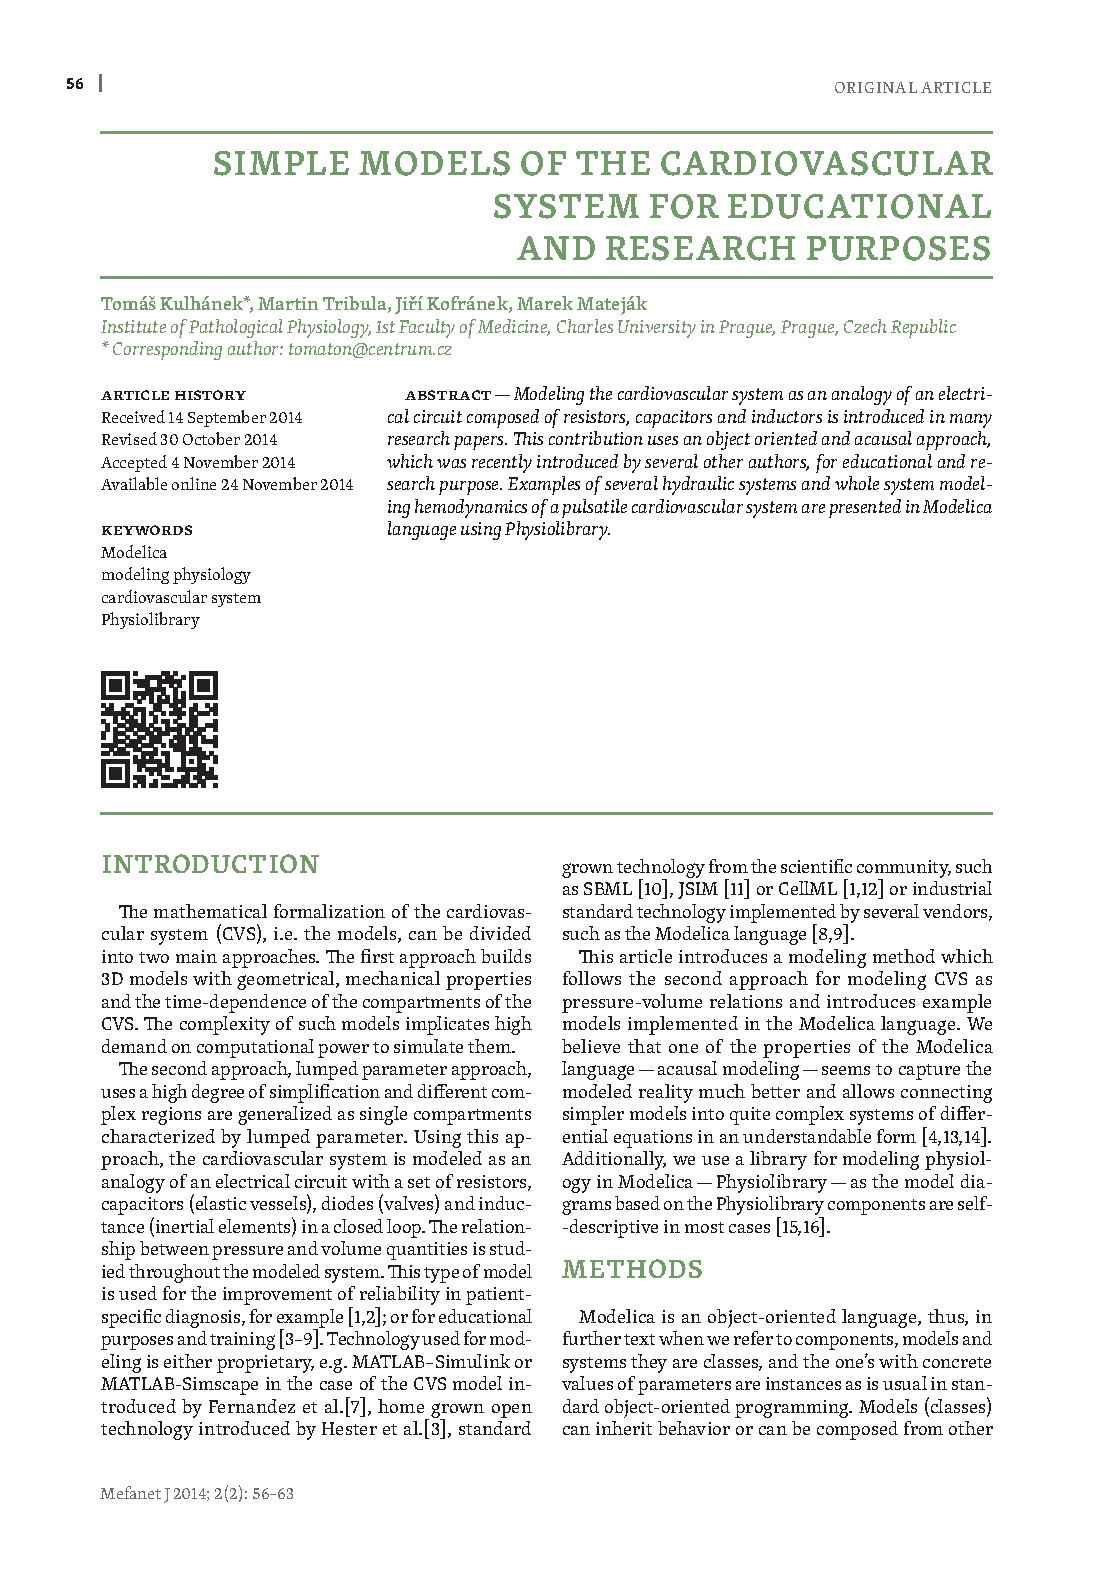
\includepdf[pages={-},pagecommand={\thispagestyle{plain}}]{appendix/mj-04140914.pdf}
{
%\fontfamily{phv}\selectfont
\makeatletter 
\renewcommand{\thefigure}{\@arabic\c@figure}
\setcounter{figure}{11}
\fontfamily{anttlc}\selectfont

\begin{figure}[ht]
    \centering
    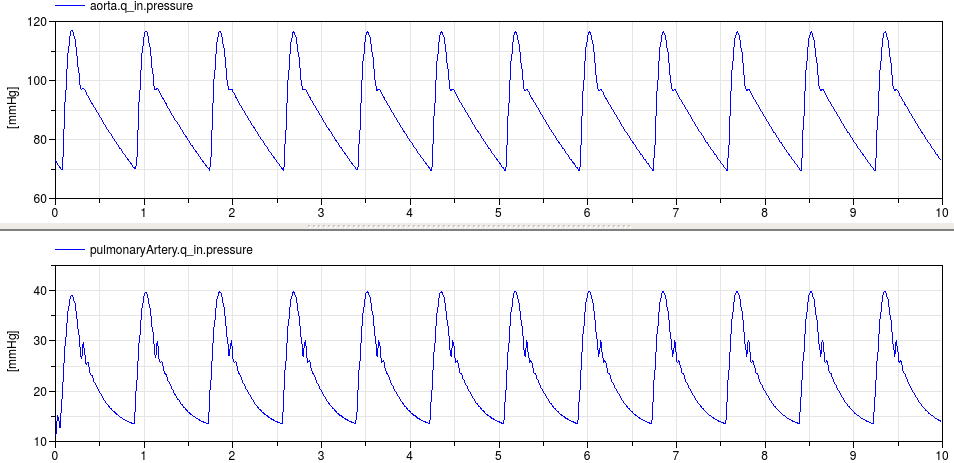
\includegraphics[width=1\textwidth]{appendix/appendix4-fig12.png}
    \caption{\fontfamily{bch}\selectfont
Pressure dynamics in systemic and pulmonary artery simulated in reference model by Fernandez de Canete et al [7].
    }
\end{figure}

\begin{figure}[ht]
    \centering
    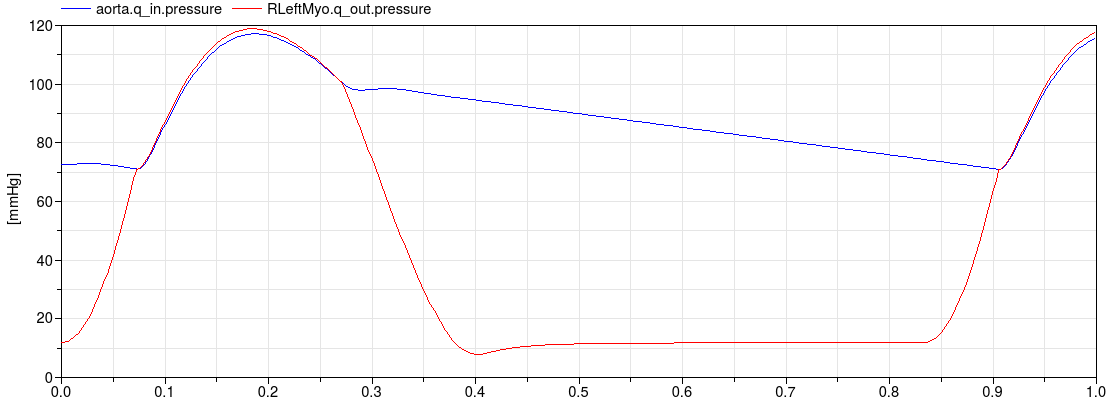
\includegraphics[width=0.8\textwidth]{appendix/appendix4-fig13.png}
    \caption{\fontfamily{bch}\selectfont
Pressure dynamics in aorta (blue) and left ventricle (red) simulated in reference model by Fernandez de Canete et al. [7]. At time 0.07s the aortic valve opens and the pressure in left ventricle is only slightly higher than in aorta allowing the blood to flow from left ventricle to aorta.
    }
\end{figure}

\begin{figure}[ht]
    \centering
    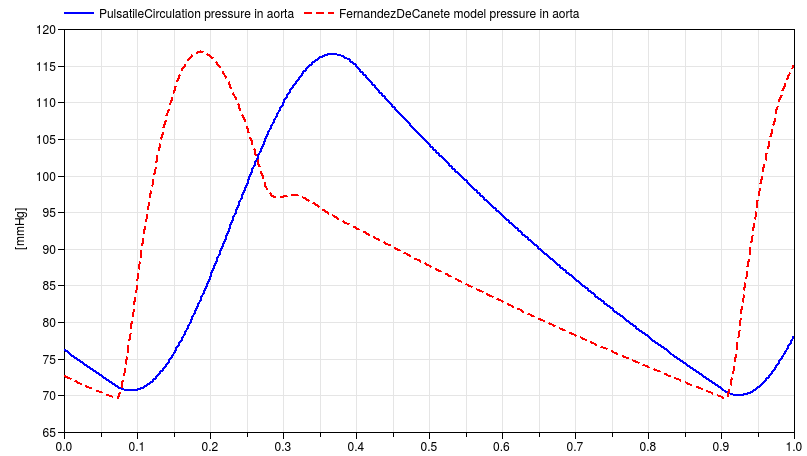
\includegraphics[width=0.8\textwidth]{appendix/appendix4-fig14.png}
    \caption{\fontfamily{bch}\selectfont
Comparison of pressure dynamics in systemic arteries simulated by simple pulsatile CVS models (blue) and by reference Fernandez de Canete model[7] implemented in Modelica (red dashed).
    }
\end{figure}

\makeatother
}